% !TeX root = thesis.tex
\chapter{Methodology}\label{C:aim}

This chapter sets out the methodological framework used throughout the thesis. We begin by explaining why entropy and complexity measures are useful for time series analysis and what their limitations are (Section~\ref{Sec:AdvantagesLimitations}), and why the ordinal pattern approach of Bandt and Pompe is our representation of choice (Section~\ref{Sec:BP method}). Section~\ref{Sec:BackgroundKnowledge} defines the information-theoretic descriptors computed from ordinal pattern distributions: permutation entropy, disequilibrium, statistical complexity, the Rényi and Tsallis entropies, and the two forms of the Fisher information measure used in this work. Section~\ref{Sec:EntropyComplexity} describes the entropy--complexity plane. Section~\ref{Sec:AsymptoticDistribution} reviews the asymptotic distribution of these descriptors, which is what allows us to attach confidence intervals to them. Section~\ref{Sec:Software} describes the two R packages on which all computations rely, and Section~\ref{Subsec:GeneralFramework} summarises the general analysis procedure. Section~\ref{Sec:Simulation} describes the design of a simulation study in which time series with known generating mechanisms are used to test whether ordinal pattern features can separate different dynamics, and Section~\ref{Sec:Clustering} presents the clustering and classification methods used in this study and in the applications. Finally, Section~\ref{Sec:Applications} explains how the same framework is applied to the two geophysical problems studied in this thesis: Synthetic Aperture Radar (SAR) time series for land cover classification and seismic amplitude data from Whakaari/White Island.

\section{Entropy and Complexity Analysis in Time Series: Advantages and Limitations}\label{Sec:AdvantagesLimitations}

Many systems of scientific interest evolve over time in ways that are neither perfectly regular nor purely random. Entropy and complexity measures give us a way to describe where a system sits between these two extremes. Shannon entropy quantifies the uncertainty of a probability distribution. Permutation entropy applies the same idea to the distribution of ordinal patterns extracted from a time series, so that it measures how diverse the order structure of the series is, rather than how spread out its values are.

Entropy on its own, however, cannot tell a structured system apart from a noisy one when both have similar entropy values. Statistical complexity was introduced to fill this gap: it combines entropy with a measure of how far the distribution is from uniform distribution, and so describes the balance between order and disorder. Used together, entropy and complexity are well suited to nonlinear dynamics, that is, systems in which outputs are not proportional to inputs and where small changes can have large or unpredictable effects. Such behaviour is common in biological, financial, climate and geophysical systems.

These measures do have practical limitations. Their values depend on the choice of parameters, in particular the embedding dimension and the time delay. They require enough data for the empirical pattern distribution to be a reliable estimate of the underlying one, and the data often need some preprocessing. Interpretation also requires knowledge of the application domain; a high entropy value is not informative unless one knows what a high value means for the system under study.

Despite these limitations, entropy and complexity measures remain valuable. Classical linear tools such as the autocorrelation function, regression and Fourier analysis assume proportional relationships and, in most cases, stationarity. Entropy and complexity measures make no such assumptions, and they are designed to respond to irregularity, changes in pattern and chaotic behaviour. This is precisely the kind of behaviour we expect in the remote sensing and volcanic data analysed later in this thesis.

\section{The Bandt and Pompe Method: A Robust Approach} \label{Sec:BP method}

Classical estimators of complexity, such as the correlation dimension~\cite{Grassberger1983}, fractal dimension and Lyapunov exponents~\cite{Wolf1985}, were developed for low-dimensional dynamical systems~\cite{Huffaker2018}. These are systems whose behaviour can be described by a small number of variables or equations, typically two or three, such as the logistic map or a simple pendulum. Although their dynamics can be rich and even chaotic, their structure is relatively easy to recover from data. The Lyapunov exponent, for example, measures the average rate at which nearby trajectories diverge or converge, and is a natural indicator of chaos in this setting. In real data, however, these estimators tend to perform poorly: they need long and clean records, and their estimates deteriorate quickly once noise is present~\cite{PhysRevLett.88.174102,Huffaker2018}.

Bandt and Pompe~\cite{PhysRevLett.88.174102} proposed a different route. Instead of working with the values of the series, they replace each short window of consecutive observations by its ordinal pattern, that is, the permutation that sorts the values in the window. The time series is thereby turned into a sequence of symbols, and all subsequent analysis is carried out on the distribution of these symbols. The main advantages of this approach are the following:
\begin{itemize}
	\item it is conceptually simple and requires no model of the data;
	\item it is computationally fast, even for very long series;
	\item it is robust to noise and to outliers, because small perturbations rarely change the order of values in a window;
	\item it is invariant under strictly increasing (monotonic) transformations of the data, so that, for instance, working with amplitudes or with their logarithms (decibels) yields the same patterns.
\end{itemize}
Because ordinal patterns are built from consecutive observations, the method also respects the temporal (causal) order of the data. These properties explain why it has been used so widely to distinguish chaotic from stochastic signals.

The method also has known shortcomings. Information about amplitude is discarded, ties between equal values must be resolved by some convention, and the number of possible patterns, $D!$, grows very quickly with the embedding dimension $D$, which increases the amount of data required. Several extensions of the original method have been proposed to address these issues. In this thesis we use the original formulation with time delay $\tau=1$ and choose $D$ so that the length of each series is large relative to $D!$.

\section{Information-Theoretic Descriptors of Ordinal Patterns} \label{Sec:BackgroundKnowledge}

Bandt and Pompe computed the Shannon entropy of the histogram of ordinal patterns and used it, among other applications, to detect chaotic components in time series. Rosso et al.~\cite{EEGAnalysisUsingWaveletBasedInformationTools} extended this analysis by adding a second dimension: the statistical complexity computed from the same histogram. Plotting one quantity against the other gives the entropy--complexity plane, which has since been used to visualise and characterise dynamical regimes as system parameters change~\cite{Bandt2005,Cao2004,DeMicco2012a,Kowalski2007,Kowalski2011b,Rosso2010a,Zunino2010a,Zunino2012a}, and has been applied to optical chaos~\cite{Liu2016f,Soriano2011a,Toomey2014,Yang2015e,Zunino2011a}, hydrology~\cite{Lange2013,Serinaldi2014,Stosic2016}, geophysics~\cite{Consolini2014,Saco2010,Sippel2016}, engineering~\cite{Aquino2017,Aquino2015,Redelico2017a,Yan2012}, biometrics~\cite{Rosso2016}, the assessment of pseudo-random number generators~\cite{DeMicco2008,DeMicco2009}, biomedical signal analysis~\cite{Li2014b,Li2008b,Li2007,Liang2015b,Montani2015a,Montani2014,Montani2014a,Montani2015,Morabito2012,Parlitz2012,Perinelli2025,Perinelli2019,Zanin2012}, and econophysics~\cite{Bariviera2015a,Bariviera2015,Bariviera2016,Zanin2012,Zunino2016a,Zunino2009,Zunino2010}, among other fields.

Closer to the problems studied in this thesis, information-theoretic descriptors have been used to track volcanic and hydrothermal activity, with permutation entropy anticipating eruptions of the Strokkur geyser~\cite{Sudibyo2022} and amplitude-based Fisher--Shannon and Shannon entropy measures revealing changes before eruptions at El Hierro and Volcán de Colima~\cite{Telesca2014,ReyDevesa2023}.
%Further in remote sensing, ordinal pattern features of Sentinel-1 SAR time series have been shown to discriminate between land cover classes~\cite{Dilhani2026SAR}.

\subsection{Notation}\label{Subsec:Notation}

We use the following notation throughout the thesis. Let $\mathbf{x}=(x_1,x_2,\dots,x_{n+D-1})$ be a real-valued time series and $D\geq 2$ the embedding dimension. For $t=1,\dots,n$ we form the overlapping windows $\mathbf{s}_t=(x_t,x_{t+1},\dots,x_{t+D-1})$ and assign to each window its ordinal pattern, as described in Chapter~\ref{C:intro}. There are $k=D!$ possible patterns, which we denote by $\pi^1,\pi^2,\dots,\pi^k$. Let $N_\ell$ be the number of windows whose pattern is $\pi^\ell$. The empirical probability function of ordinal patterns is then
\begin{equation}
	\widehat{\mathbf{p}}=\left(\frac{N_1}{n},\frac{N_2}{n},\dots,\frac{N_k}{n}\right)=(\widehat{p}_1,\widehat{p}_2,\dots,\widehat{p}_k),
	\label{eq:EmpiricalP}
\end{equation}
which estimates the true (unknown) probability function $\mathbf{p}=(p_1,\dots,p_k)$. All descriptors below are written for a generic probability function $\mathbf{p}$; in practice they are evaluated at $\widehat{\mathbf{p}}$. Throughout, $\log$ denotes the natural logarithm and we adopt the convention $0\log 0=0$.

\subsection{Permutation entropy}

The Shannon entropy of $\mathbf{p}$ is
\begin{equation}
	S(\mathbf{p})=-\sum_{\ell=1}^{k}p_\ell\log p_\ell ,
	\label{eq:ShannonUnnorm}
\end{equation}
and its normalised version,
\begin{equation}
	H(\mathbf{p})=\frac{S(\mathbf{p})}{\log k}=-\frac{1}{\log k}\sum_{\ell=1}^{k}p_\ell\log p_\ell ,
	\label{eq:NormShannon}
\end{equation}
is known as the permutation entropy when $\mathbf{p}$ is an ordinal pattern distribution. The normalisation keeps the entropy in the unit interval, which allows comparisons across embedding dimensions:
\begin{itemize}
	\item $H(\mathbf{p})=0$ when a single pattern occurs, i.e., $p_\ell=1$ for some $\ell$;
	\item $H(\mathbf{p})=1$ when all patterns are equally likely, i.e., $p_\ell=1/k$ for every $\ell$.
\end{itemize}
Low values therefore indicate regular, predictable dynamics, while values close to one indicate that the order structure is close to random.

\subsection{Disequilibrium and statistical complexity}

Permutation entropy measures disorder, but it cannot fully characterise the dynamics: quite different processes can have similar entropy. López-Ruiz et al.~\cite{lopez1995statistical} addressed this by introducing the disequilibrium $Q$, which measures how far $\mathbf{p}$ is from the uniform, non-informative distribution $\mathbf{u}=(1/k,\dots,1/k)$. In their original proposal the distance was Euclidean. Lamberti et al.~\cite{lamberti2004intensive} replaced it with the Jensen--Shannon divergence, which is symmetric, bounded, and has a clear information-theoretic meaning:
\begin{equation}
	J(\mathbf{p},\mathbf{u})=S\!\left(\frac{\mathbf{p}+\mathbf{u}}{2}\right)-\frac{1}{2}S(\mathbf{p})-\frac{1}{2}S(\mathbf{u}),
	\label{eq:JSD}
\end{equation}
where $S(\mathbf{u})=\log k$. The divergence attains its maximum when all the probability is concentrated on a single pattern, in which case
\begin{equation}
	J_{\max}=-\frac{1}{2}\left[\frac{k+1}{k}\log(k+1)-2\log(2k)+\log k\right].
	\label{eq:JSDmax}
\end{equation}
The normalised disequilibrium is
\begin{equation}
	Q(\mathbf{p})=\frac{J(\mathbf{p},\mathbf{u})}{J_{\max}},
	\label{eq:Disequilibrium}
\end{equation}
which equals zero for the uniform distribution and one for a degenerate distribution. Following Lamberti et al.~\cite{lamberti2004intensive}, the statistical complexity is the product
\begin{equation}
	C(\mathbf{p})=H(\mathbf{p})\,Q(\mathbf{p}).
	\label{eq:Complexity}
\end{equation}
Since both factors lie in $[0,1]$, so does $C$. The product form means that complexity is small at both extremes, perfect order ($H=0$) and complete randomness ($Q=0$), and is largest for distributions that combine moderate disorder with marked structure. To make clear which information measure it is built on, we also write $C_S=HQ$ and call it the Shannon complexity.

\subsection{Rényi and Tsallis entropies}

Shannon entropy weights every pattern by its probability. Generalised entropies introduce a parameter $q$ that changes this weighting, giving more or less importance to rare patterns. The Rényi entropy~\cite{renyi1961measures} is
\begin{equation}
	H_{R}^{q}(\mathbf{p})=\frac{1}{1-q}\log\sum_{\ell=1}^{k}p_\ell^{\,q},\qquad q\in\mathbb{R}^{+}\setminus\{1\},
	\label{eq:Renyi}
\end{equation}
and the Tsallis entropy~\cite{tsallis1988possible} is
\begin{equation}
	H_{T}^{q}(\mathbf{p})=\sum_{\ell=1}^{k}\frac{p_\ell-p_\ell^{\,q}}{q-1},\qquad q\in\mathbb{R}\setminus\{1\}.
	\label{eq:Tsallis}
\end{equation}
Both reduce to the Shannon entropy~\eqref{eq:ShannonUnnorm} in the limit $q\to1$. Values $q<1$ emphasise rare patterns and values $q>1$ emphasise dominant ones. In our applications we use $q=1.5$, in line with the value used by Rey et al.~\cite{Rey2023}.

As with the Shannon entropy, both quantities are normalised by their value under the uniform distribution, which is their maximum:
\begin{equation}
	\widetilde{H}_{R}^{q}(\mathbf{p})=\frac{H_{R}^{q}(\mathbf{p})}{\log k},
	\qquad
	\widetilde{H}_{T}^{q}(\mathbf{p})=\frac{(q-1)\,H_{T}^{q}(\mathbf{p})}{1-k^{1-q}},
	\label{eq:NormRenyiTsallis}
\end{equation}
so that both lie in $[0,1]$. Replacing $H$ by $\widetilde{H}_{R}^{q}$ or $\widetilde{H}_{T}^{q}$ in~\eqref{eq:Complexity}, while keeping the same disequilibrium $Q$, gives the Rényi complexity $C_R=\widetilde{H}_{R}^{q}\,Q$ and the Tsallis complexity $C_T=\widetilde{H}_{T}^{q}\,Q$.

\subsection{Fisher information measure}\label{Subsec:Fisher}

The Fisher information~\cite{frieden2004science} was originally defined for continuous densities as the expected squared derivative of the log-density. It therefore measures how sharply a distribution changes, rather than how spread out it is. This makes it a local measure, in contrast with Shannon entropy, which is global: entropy is unchanged by any reordering of the probabilities, whereas the Fisher information responds to differences between neighbouring probabilities. As a consequence, it is more sensitive to small changes and perturbations in the pattern distribution.

For a discrete distribution, the derivative is replaced by differences between consecutive probabilities. Two discretisations appear in the literature, and both are used in this thesis.

\paragraph{Form 1: square-root (Hellinger-type) discretisation.} Following Sánchez-Moreno et al.~\cite{sanchez2009discrete}, the first form is
\begin{equation}
	F_1(\mathbf{p})=F_0\sum_{\ell=1}^{k-1}\left(\sqrt{p_{\ell+1}}-\sqrt{p_\ell}\right)^2,
	\label{eq:Fisher1}
\end{equation}
where $F_0$ is a normalisation constant. In this thesis we use $F_0=4$, the constant adopted by Rey et al.~\cite{Rey2024} in their derivation of the asymptotic distribution of the Fisher information of ordinal patterns. Working with square roots of probabilities avoids divisions by zero when some patterns are not observed, and it is the form for which asymptotic results are available (Section~\ref{Subsec:OtherAsymptotics}).

\paragraph{Form 2: difference-ratio discretisation.} The second form, proposed by Ferri et al.~\cite{Ferri2009} and used in our study of SAR land cover, is
\begin{equation}
	F_2(\mathbf{p})=\frac{1}{4}\sum_{\ell=1}^{k-1}\frac{2\,(p_{\ell+1}-p_\ell)^2}{p_{\ell+1}+p_\ell}
	=\frac{1}{2}\sum_{\ell=1}^{k-1}\frac{(p_{\ell+1}-p_\ell)^2}{p_{\ell+1}+p_\ell},
	\label{eq:Fisher2}
\end{equation}
where terms with $p_{\ell+1}+p_\ell=0$ are taken as zero. In the implementation, a small constant ($10^{-12}$) is added to the denominator to avoid numerical division by zero.

\paragraph{Relation between the two forms.} The two forms are closely related. Since $(\sqrt{a}-\sqrt{b})^2=(a-b)^2/(\sqrt{a}+\sqrt{b})^2$, and $a+b\leq(\sqrt{a}+\sqrt{b})^2\leq 2(a+b)$ for $a,b\geq 0$, each term of~\eqref{eq:Fisher1} lies between one half and one times the corresponding term of $\sum (p_{\ell+1}-p_\ell)^2/(p_{\ell+1}+p_\ell)$. Hence
\begin{equation}
	F_2(\mathbf{p})\;\leq\;\frac{F_1(\mathbf{p})}{F_0}\;\leq\;2\,F_2(\mathbf{p}).
	\label{eq:FisherBounds}
\end{equation}
The two measures therefore carry essentially the same information about local changes in the distribution, but they are on different scales and are not interchangeable. For this reason we always state which form is being used, and we never compare numerical values of $F_1$ with values of $F_2$.

A feature shared by both forms is that, unlike the entropies, they depend on the order in which the $k$ patterns are listed. Olivares et al.~\cite{Olivares2012b} discussed this ambiguity and showed that different ordering schemes can lead to different values. The ordering is fixed by the software used to enumerate the patterns, and we keep the same ordering within each analysis so that results are comparable.

\paragraph{Fisher complexity.} By analogy with~\eqref{eq:Complexity}, we define the Fisher complexity as
\begin{equation}
	C_F(\mathbf{p})=F(\mathbf{p})\,Q(\mathbf{p}),
	\label{eq:FisherComplexity}
\end{equation}
where $F$ is whichever Fisher form is used in the analysis at hand. Plotting $C_F$ against $F$ gives the Fisher information--complexity plane, which we use alongside the entropy--complexity plane.

\section{The Entropy--Complexity Plane} \label{Sec:EntropyComplexity}

The entropy--complexity plane, also written $H\times C$, is a two-dimensional representation in which each time series is placed according to the permutation entropy and statistical complexity of its ordinal pattern distribution. For a given embedding dimension $D$, not every point of the unit square can be reached, and the location of a series within the feasible region says a great deal about its dynamics.

\subsection{Key dynamics in the plane}

Two extreme cases help to read the plane.
\begin{enumerate}
	\item \textbf{Highly ordered systems}, whose behaviour is predictable and often repeats regularly. A strictly monotonic series, for example, produces a single ordinal pattern. Its entropy is $H=0$, its disequilibrium is maximal ($Q=1$), and so its complexity is $C=0$. It is mapped to the point $(0,0)$.
	\item \textbf{Completely random systems}. White noise produces all patterns with equal probability, so that $H=1$ and the disequilibrium vanishes ($Q=0$). It is mapped to the point $(1,0)$: maximal entropy and no structure.
\end{enumerate}
The existence of these extreme values was established by Anteneodo and Plastino~\cite{anteneodo1996some}. Between them, deterministic chaotic systems tend to occupy the upper part of the region, with intermediate entropy and high complexity, whereas correlated stochastic processes lie closer to the lower boundary.

Martin et al.~\cite{Martin2006} derived the boundaries of the feasible region using geometrical arguments in the space of probability functions. The lower boundary is a smooth curve, whereas the upper boundary consists of $D!-1$ separate segments; as $D$ increases, the upper boundary approaches a smooth curve. Figure~\ref{fig:complexity} shows the feasible region for embedding dimensions $3$ to $6$. Figure~\ref{fig:tentimeseries} shows ten time series together with their positions in the $H\times C$ plane for $D=6$.

\begin{figure}[H]
	\centering
	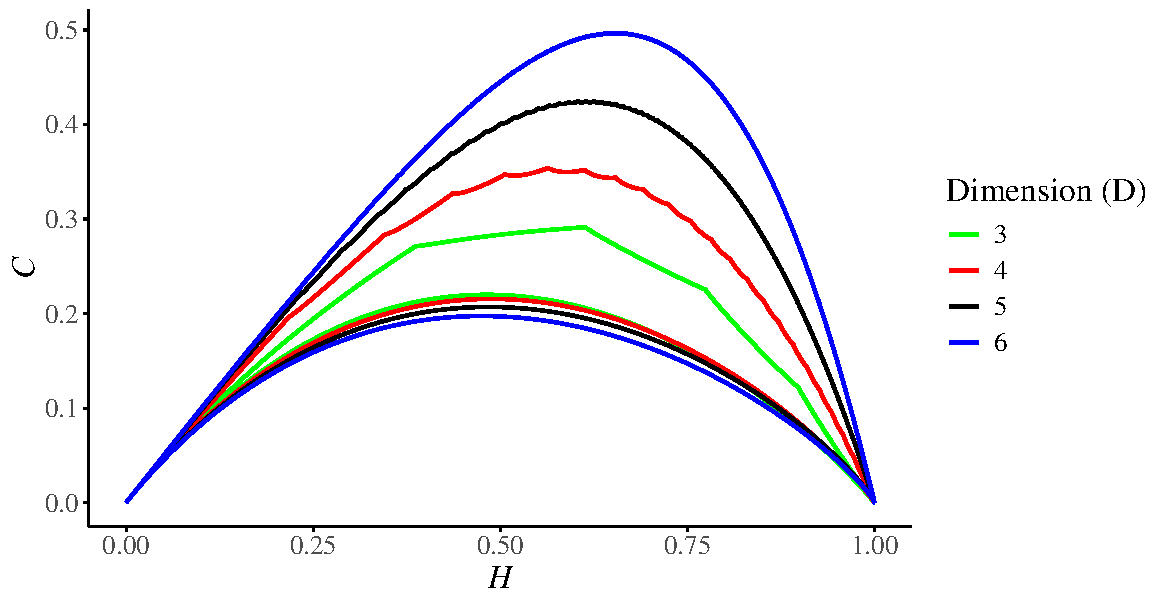
\includegraphics[width=0.7\textwidth]{Figures/Chapter3/complexity plane}
	\caption{Feasible region of the entropy--complexity plane for embedding dimensions $D=3,4,5$ and $6$.}
	\label{fig:complexity}
\end{figure}

\begin{figure}[H]
	\centering
	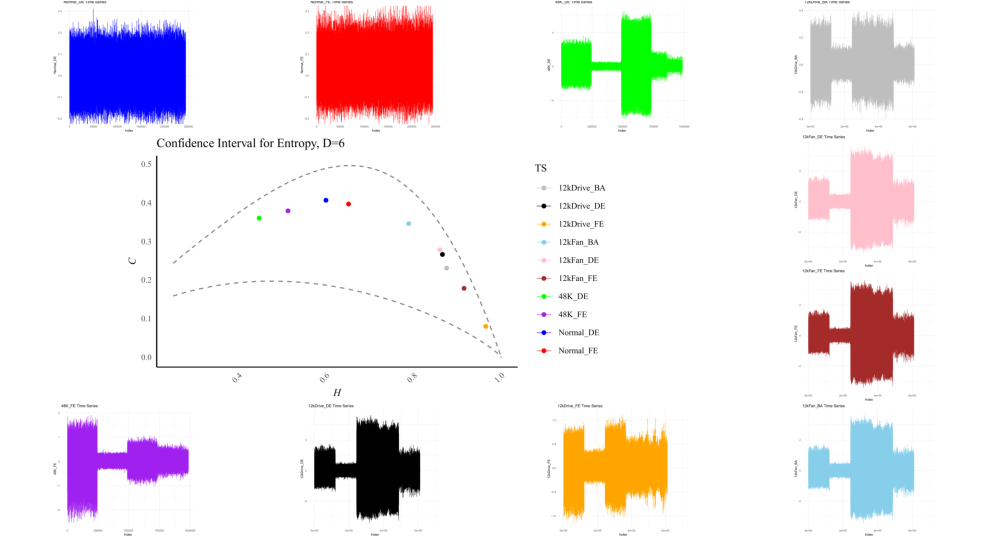
\includegraphics[width=0.7\textwidth]{Figures/Chapter3/combined plot}
	\caption{Ten time series and their positions in the $H\times C$ plane for embedding dimension $D=6$.}
	\label{fig:tentimeseries}
\end{figure}

Unlike the entropy--complexity plane, the Fisher information--complexity plane has no known closed-form boundaries, so we use it as a descriptive tool rather than one with a fixed reference frame.

\section{Asymptotic Distribution of Ordinal Pattern Descriptors}\label{Sec:AsymptoticDistribution}

Every descriptor in Section~\ref{Sec:BackgroundKnowledge} is computed from the estimate $\widehat{\mathbf{p}}$ and is therefore a random quantity. Two series may produce different entropy values simply because of sampling variability, so to compare series in a meaningful way we need to know how much these descriptors vary. The exact distribution of these statistics is difficult to obtain, and the literature has approached the problem in two ways.

The first approach is empirical. Here one simulates or resamples many series from a model and builds the distribution of the descriptors directly from the resulting values. Combined with knowledge of the expected variability of entropy and complexity, this allows hypothesis tests for a wide range of models~\cite{Chagas2022a,DeMicco2008,Larrondo2005,Larrondo2006}. Its drawback is that it requires a model and can be computationally expensive.

The second approach, which we follow, is asymptotic. It gives closed-form approximations of the variance that hold when the number of patterns $n$ is large. Two models are considered. In the \emph{multinomial model}, the patterns are treated as independent draws from $\mathbf{p}$. This is a convenient simplification, but it is not strictly true: consecutive windows overlap in $D-1$ observations, so neighbouring patterns are dependent. The second model accounts for this \emph{serial dependence}.

\subsection{Asymptotic distribution of the Shannon entropy under the multinomial model}\label{Subsec:Multinomial}

Under the multinomial model, the vector of counts $\mathbf{N}=(N_1,\dots,N_k)$, with $\sum_{\ell}N_\ell=n$, follows a multinomial distribution $\mathbf{N}\sim\mathrm{Mult}(n,\mathbf{p})$ with probability mass function
\[
\Pr(\mathbf{N}=\mathbf{m})=n!\prod_{\ell=1}^{k}\frac{p_\ell^{m_\ell}}{m_\ell!},
\]
and moments
\[
\mathrm{E}(N_\ell)=np_\ell,\qquad
\mathrm{Var}(N_\ell)=np_\ell(1-p_\ell),\qquad
\mathrm{Cov}(N_\ell,N_j)=-np_\ell p_j \quad (\ell\neq j).
\]
The maximum likelihood estimator of $p_\ell$ is $\widehat{p}_\ell=N_\ell/n$, which is exactly~\eqref{eq:EmpiricalP}. By the invariance property of maximum likelihood estimators, $g(\widehat{\mathbf{p}})$ is the maximum likelihood estimator of $g(\mathbf{p})$ for any function $g$; in particular, $S(\widehat{\mathbf{p}})$ estimates $S(\mathbf{p})$. Written in terms of the counts,
\begin{align}
	S(\widehat{\mathbf{p}})
	&=-\sum_{\ell=1}^{k}\frac{N_\ell}{n}\log\frac{N_\ell}{n}
	=\log n-\frac{1}{n}\sum_{\ell=1}^{k}N_\ell\log N_\ell .
	\label{eq:AsymEntropy}
\end{align}
The unnormalised entropy lies between $0$ and $\log k$; the minimum is attained when $p_\ell=1$ for some $\ell$ and $p_j=0$ for all $j\neq\ell$, and the maximum when $p_\ell=1/k$ for every $\ell$.

The asymptotic behaviour of $S(\widehat{\mathbf{p}})$ follows from that of $\widehat{\mathbf{p}}$. Define $\mathbf{Y}_n=\sqrt{n}\,(\widehat{\mathbf{p}}-\mathbf{p})$. Then $\mathrm{E}(\mathbf{Y}_n)=\mathbf{0}$ and $\mathrm{Cov}(\mathbf{Y}_n)=\mathbf{D_p}-\mathbf{p}\mathbf{p}^{T}$, where $\mathbf{D_p}=\mathrm{Diag}(p_1,\dots,p_k)$ and $T$ denotes transposition. By the multivariate central limit theorem,
\begin{equation}
	\mathbf{Y}_n\xrightarrow{\mathscr{D}}N_k\!\left(\mathbf{0},\,\mathbf{D_p}-\mathbf{p}\mathbf{p}^{T}\right),
	\label{eq:Cov}
\end{equation}
where the covariance matrix has entries
\begin{equation}
	\left(\mathbf{D_p}-\mathbf{p}\mathbf{p}^{T}\right)_{\ell j}=
	\begin{cases}
		p_\ell(1-p_\ell), & \text{if } \ell=j,\\[4pt]
		-\,p_\ell p_j, & \text{if } \ell\neq j,
	\end{cases}
	\qquad 1\leq\ell,j\leq k.
	\label{eq:CovEntries}
\end{equation}
To transfer this result to a function of $\widehat{\mathbf{p}}$, such as the entropy, we refer to the Delta method.

\theoremstyle{plain}
\newtheorem{theorem}{Theorem}

\begin{theorem}[Delta method, univariate]
	Let $(X_n)$ be a sequence of random variables such that $\sqrt{n}\,(X_n-\theta)\xrightarrow{\mathscr{D}}N(0,\sigma^2)$, and let $h$ be a function such that $h'(\theta)$ exists and $h'(\theta)\neq0$. Then
	\[
	\sqrt{n}\,\big[h(X_n)-h(\theta)\big]\xrightarrow{\mathscr{D}}N\!\left(0,\,\sigma^2\,[h'(\theta)]^2\right).
	\]
\end{theorem}

\begin{theorem}[Delta method, multivariate]
	Let $(\mathbf{X}_n)$ be a sequence of random vectors in $\mathbb{R}^k$ such that $\sqrt{n}\,(\mathbf{X}_n-\boldsymbol{\theta})\xrightarrow{\mathscr{D}}N_k(\mathbf{0},\Sigma)$. Let $h\colon\mathbb{R}^k\to\mathbb{R}^m$ be continuously differentiable in a neighbourhood of $\boldsymbol{\theta}$, with $m\times k$ Jacobian matrix $B=\left(\partial h_i/\partial\theta_j\right)$ evaluated at $\boldsymbol{\theta}$, and assume $B\Sigma B^{T}$ is non-singular. Then
	\[
	\sqrt{n}\,\big(h(\mathbf{X}_n)-h(\boldsymbol{\theta})\big)\xrightarrow{\mathscr{D}}N_m\!\left(\mathbf{0},\,B\Sigma B^{T}\right).
	\]
\end{theorem}

Applying the multivariate Delta method with $h=S$, whose partial derivatives are $\partial S/\partial p_\ell=-(\log p_\ell+1)$, and using~\eqref{eq:CovEntries}, Rey et al.~\cite{Rey2023,Rey2025} showed that $S(\widehat{\mathbf{p}})$ is asymptotically normal with mean $S(\mathbf{p})$ and variance $\sigma^2_{\mathbf{p}}/n$, where
\begin{equation}
	\sigma^2_{\mathbf{p}}=\sum_{\ell=1}^{k}p_\ell(1-p_\ell)(\log p_\ell+1)^2-2\sum_{j=1}^{k-1}\sum_{\ell=j+1}^{k}p_\ell p_j(\log p_\ell+1)(\log p_j+1).
	\label{eq:SigmaMultinomial}
\end{equation}
In practice $\mathbf{p}$ is unknown and is replaced by $\widehat{\mathbf{p}}$, giving the plug-in estimate $\widehat{\sigma}^2_{\widehat{\mathbf{p}}}$. Because the normalised entropy~\eqref{eq:NormShannon} is $S/\log k$, its asymptotic variance is $\sigma^2_{\mathbf{p}}/(n\log^2 k)$.

Rey et al.~\cite{Rey2025} went further and derived the asymptotic distribution of the statistical complexity under the multinomial model. They showed that it also converges to a normal distribution, with a variance and bias that reflect the underlying dynamics, and their numerical studies indicate that the approximation remains useful when the multinomial assumption is only approximately satisfied, as is the case for Bandt--Pompe patterns.

\subsection{Asymptotic distribution of the permutation entropy under pattern dependence}\label{Subsec:PatternDependence}

The multinomial model ignores the fact that the windows $\mathbf{s}_t$ and $\mathbf{s}_{t+r}$ share observations whenever $r<D$. As a result, the pattern at time $t$ restricts which patterns can appear at times $t+1,\dots,t+D-1$, and the patterns are dependent. Rey et al.~\cite{Rey2023a} derived the asymptotic variance of the entropy under this dependence.

For $r=1,\dots,D-1$, let $p^{(r)}_{ij}$ denote the probability of observing pattern $\pi^j$ at time $t+r$ given pattern $\pi^i$ at time $t$, and collect these transition probabilities in the matrix $\mathbf{Q}^{(r)}=\big(p^{(r)}_{ij}\big)$. When $n$ is sufficiently large, the asymptotic variance of the Shannon entropy is
\begin{equation}
	\begin{split}
		\widehat{\nu}^2_{\widehat{\mathbf{p}}} = \widehat{\sigma}^2_{\widehat{\mathbf{p}}}
		& + \sum_{i=1}^{k}(\log \widehat{p}_i + 1)^2
		\left[ (2D - 2)\,\widehat{p}_i^{\,2} + 2\sum_{r=1}^{D-1} \mathbf{Q}^{(r)}_{ii} \right] \\
		& - 2 \sum_{i=1}^{k-1} \sum_{j=i+1}^{k} (\log \widehat{p}_i + 1)(\log \widehat{p}_j + 1)
		\left[ (2D - 1)\,\widehat{p}_i \widehat{p}_j - \sum_{r=1}^{D-1} \left( \mathbf{Q}^{(r)}_{ij} + \mathbf{Q}^{(r)}_{ji} \right) \right],
	\end{split}
	\label{eq:asympvar}
\end{equation}
where the first term is the multinomial variance~\eqref{eq:SigmaMultinomial} and the remaining terms correct for the overlap between windows.

For practical purposes, and for $n$ sufficiently large, the entropy estimator can be approximated by a normal distribution with mean $S(\widehat{\mathbf{p}})$ and variance $\widehat{\nu}^2_{\widehat{\mathbf{p}}}/n$. For $\alpha\in(0,1)$, an approximate $(1-\alpha)\times100\%$ confidence interval for the entropy is therefore
\begin{equation}
	S(\widehat{\mathbf{p}})\pm z_{1-\alpha/2}\,\frac{\widehat{\nu}_{\widehat{\mathbf{p}}}}{\sqrt{n}},
	\label{eq:ConfidenceInterval}
\end{equation}
where $z_{1-\alpha/2}$ is the $(1-\alpha/2)$-quantile of the standard normal distribution ($z_{0.975}\approx1.96$ for a $95\%$ interval). The same interval is obtained under the multinomial model by replacing $\widehat{\nu}_{\widehat{\mathbf{p}}}$ with $\widehat{\sigma}_{\widehat{\mathbf{p}}}$. For brevity we write the interval as
\begin{equation}
	S(\widehat{\mathbf{p}})\pm\text{semi-length},\qquad
	\text{semi-length}=z_{1-\alpha/2}\,\frac{\widehat{\nu}_{\widehat{\mathbf{p}}}}{\sqrt{n}},
	\label{eq:CI}
\end{equation}
and, for the normalised entropy $H$, both the estimate and the semi-length are divided by $\log k$.

\subsection{Asymptotic variance of the statistical complexity}\label{Subsec:AsympVarComplexity}

The variance of $C(\widehat{\mathbf{p}})$ is obtained in the same way, by applying the multivariate Delta method to $C=HQ$. This follows Rey et al.~\cite{Rey2025}, and the joint asymptotic behaviour of entropy and disequilibrium has recently been studied by Silbernagel et al.~\cite{silbernagel2025joint}. We consider two estimators of the variance:
\begin{itemize}
	\item the \textbf{multinomial variance}, $\widehat{\omega}^2_{\widehat{\mathbf{p}}}$, which assumes independent patterns; and
	\item the \textbf{serial dependence variance}, $\widehat{\eta}^2_{\widehat{\mathbf{p}}}$, which accounts for overlapping windows.
\end{itemize}

\paragraph{Multinomial model.} Under independence, the estimator is asymptotically normal,
\[
\sqrt{n}\,\big(C(\widehat{\mathbf{p}})-C(\mathbf{p})\big)\xrightarrow{\mathscr{D}}N\!\left(0,\,\omega^2_{\mathbf{p}}\right),
\qquad
\omega^2_{\mathbf{p}}=\nabla C(\mathbf{p})^{T}\,\Sigma\,\nabla C(\mathbf{p}),
\]
with $\Sigma=\mathbf{D_p}-\mathbf{p}\mathbf{p}^{T}$. By the product rule, the gradient has components
\[
\frac{\partial C}{\partial p_\ell}=Q(\mathbf{p})\frac{\partial H}{\partial p_\ell}+H(\mathbf{p})\frac{\partial Q}{\partial p_\ell},
\]
where, differentiating~\eqref{eq:NormShannon} and~\eqref{eq:JSD},
\[
\frac{\partial H}{\partial p_\ell}=-\frac{\log p_\ell+1}{\log k},
\qquad
\frac{\partial Q}{\partial p_\ell}=\frac{1}{2J_{\max}}\log\frac{2p_\ell}{p_\ell+1/k}.
\]
Because every row of $\Sigma$ sums to zero, adding a constant to all components of the gradient does not change $\omega^2_{\mathbf{p}}$; this is why the constraint $\sum_\ell p_\ell=1$ does not need to be imposed explicitly. The plug-in estimate $\widehat{\omega}^2_{\widehat{\mathbf{p}}}$ is obtained by evaluating all quantities at $\widehat{\mathbf{p}}$. These expressions are implemented in the \texttt{StatOrdPattHxC} package (Section~\ref{Sec:Software}).

\paragraph{Serial dependence.} When patterns are dependent, the variance of the complexity increases, just as that of the entropy does. In this thesis we approximate this increase by assuming that the dependence inflates the variance of the complexity by the same factor as the variance of the entropy:
\begin{equation}
	\widehat{\eta}^2_{\widehat{\mathbf{p}}}=a\,\widehat{\omega}^2_{\widehat{\mathbf{p}}},
	\qquad
	a=\frac{\widehat{\nu}^2_{\widehat{\mathbf{p}}}}{\widehat{\sigma}^2_{\widehat{\mathbf{p}}}},
	\label{eq:EtaApprox}
\end{equation}
where $\widehat{\nu}^2_{\widehat{\mathbf{p}}}$ and $\widehat{\sigma}^2_{\widehat{\mathbf{p}}}$ are the entropy variances under dependence~\eqref{eq:asympvar} and independence~\eqref{eq:SigmaMultinomial}, respectively. Combining these results,
\[
\mathrm{Var}\big(C(\widehat{\mathbf{p}})\big)\approx\frac{\widehat{\eta}^2_{\widehat{\mathbf{p}}}}{n}
=\frac{a}{n}\,\nabla C(\widehat{\mathbf{p}})^{T}\,\widehat{\Sigma}\,\nabla C(\widehat{\mathbf{p}}).
\]
We stress that~\eqref{eq:EtaApprox} is a practical approximation rather than an exact result, and confidence intervals for the complexity under dependence should be read with this in mind.

\subsection{Asymptotic results for other descriptors}\label{Subsec:OtherAsymptotics}

Asymptotic results are also available for the other descriptors used in this thesis. Under the multinomial model, the Rényi and Tsallis entropies have well-established asymptotic properties~\cite{Pardo1997,Rey2023,Rey2024}: their sample versions are asymptotically normal, and explicit expressions for the asymptotic mean and variance allow confidence intervals to be built in the same way as for the Shannon entropy~\cite{Pardo1997,Rey2024}. Rey et al.~\cite{Rey2023,Rey2024} obtained the corresponding result for the Fisher information measure in its square-root form~\eqref{eq:Fisher1}~\cite{Bobkov2019}. These results rely on the plug-in estimate $\widehat{\mathbf{p}}$ and hold under large-sample conditions and mild regularity assumptions, such as all $p_\ell$ being positive.

We are not aware of a comparable asymptotic result for the difference-ratio form~\eqref{eq:Fisher2}. For this reason, when uncertainty quantification is needed we use $F_1$, and we use $F_2$ only as a descriptive feature, as in the simulation study of Section~\ref{Sec:Simulation} and the land cover classification of Section~\ref{Subsec:SARApplication}.

\section{Computational Implementation}\label{Sec:Software}

All computations in this thesis were carried out in R, using two packages that implement ordinal pattern analysis. We describe them here so that the analyses in later chapters can be reproduced.

\subsection{The \texttt{StatOrdPattHxC} package}

The \texttt{StatOrdPattHxC} package (version~0.1)~\cite{StatOrdPattHxC} was developed by A.A. Rey and A.C. Frery and is distributed through GitHub. It accompanies the theoretical work of Rey et al.~\cite{Rey2025,Rey2023a,Rey2024,Rey2023} and implements the asymptotic results of Section~\ref{Sec:AsymptoticDistribution}. In this thesis we use it for the following tasks:
\begin{itemize}
	\item computing the Rényi and Tsallis entropies (\texttt{HRenyi}, \texttt{HTsallis});
	\item computing asymptotic variances of the entropies under the multinomial model (\texttt{asymptoticVarHShannonMultinomial}, \texttt{sigma2q});
	\item computing the asymptotic mean and variance of the statistical complexity (\texttt{meanC}, \texttt{varC});
	\item drawing the boundaries of the entropy--complexity plane, for which the package provides the \texttt{LinfLsup} data set with the lower and upper limit curves for each embedding dimension.
\end{itemize}

\subsection{The \texttt{ordinalpatterns} package}

The \texttt{ordinalpatterns} package (version~0.2.5) provides the basic tools for turning a time series into an ordinal pattern distribution and computing descriptors from it. We use the following functions:
\begin{itemize}
	\item \texttt{op\_pd}, which returns the ordinal pattern probability function $\widehat{\mathbf{p}}$ as a vector of length $D!$, including zeros for patterns that are not observed;
	\item \texttt{permutation\_entropy} (with \texttt{normalized = TRUE}), which returns $H(\widehat{\mathbf{p}})$;
	\item \texttt{statistical\_complexity}, which returns $C(\widehat{\mathbf{p}})$;
	\item \texttt{fisher\_information}, which returns the Fisher information measure;
	\item \texttt{pjsd}, which returns the Jensen--Shannon divergence.
\end{itemize}
The Jensen--Shannon divergence in this package is computed with natural logarithms; when a value in $[0,1]$ is required, it is divided by $\log 2$ or by $J_{\max}$ as in~\eqref{eq:Disequilibrium}.

\subsection{Combining the two packages}

The two packages overlap in part, and we use each for what it does best. The ordinal pattern distribution $\widehat{\mathbf{p}}$ is computed once with \texttt{ordinalpatterns}, and the same vector is passed to the functions of \texttt{StatOrdPattHxC}. This guarantees that all descriptors of a given series, and their variances, are computed from exactly the same distribution and the same ordering of patterns, which matters for the Fisher information. To avoid conflicts between functions with similar names, every call is written with an explicit namespace (for example, \texttt{StatOrdPattHxC::varC}). Unless stated otherwise, we use time delay $\tau=1$, Tsallis and Rényi index $q=1.5$, and $95\%$ confidence intervals ($z_{0.975}=1.96$). The embedding dimension depends on the application and is stated in each case. As a rule, a window is analysed only if it contains at least $5\cdot D!$ patterns, so that the pattern distribution can be estimated reliably.

\section{General Analysis Procedure}\label{Subsec:GeneralFramework}

The descriptors, the two planes and the asymptotic confidence intervals described above are combined into the following procedure, which we follow in the rest of the thesis.
\begin{enumerate}
	\item \textbf{Compute the pattern distribution.} Choose $D$ and $\tau$, divide the series into the windows of interest, and compute $\widehat{\mathbf{p}}$ for each window.
	\item \textbf{Compute the descriptors.} Calculate entropy and complexity, together with the other descriptors required by the application (Rényi and Tsallis entropies, Fisher information and Fisher complexity).
	\item \textbf{Quantify uncertainty.} Use the asymptotic variances of Section~\ref{Sec:AsymptoticDistribution} to build confidence intervals, preferring the serial dependence variance whenever it is available.
	\item \textbf{Plot.} Place each window in the $H\times C$ plane (entropy on the horizontal axis, complexity on the vertical axis) together with the feasible region for the chosen $D$, and add the confidence intervals. The $F\times C_F$ plane is plotted in the same way.
	\item \textbf{Interpret.} Read the position of each point using the general guide in Table~\ref{tab:PlaneInterpretation}.
	\item \textbf{Compare.} When the confidence intervals of two windows or groups do not overlap, this is evidence of a significant difference between them. Overlapping intervals do not, on their own, prove that the two are the same; they only indicate that the data do not show a clear difference.
	\item \textbf{Group.} When many series or windows are analysed together, use the descriptors as a feature vector for clustering or classification (Section~\ref{Sec:Clustering}).
\end{enumerate}

\begin{table}[H]
	\centering
	\begin{tabular}{ll}
		\toprule
		Region of the plane & Typical interpretation \\
		\midrule
		High $H$, low $C$ & Random or noise-dominated dynamics \\
		Intermediate $H$, high $C$ & Structured, complex dynamics (e.g.\ chaos) \\
		Low $H$, low $C$ & Simple, highly predictable dynamics \\
		\bottomrule
	\end{tabular}
	\caption{General guide to reading the entropy--complexity plane.}
	\label{tab:PlaneInterpretation}
\end{table}

\section{Simulation Study Design}\label{Sec:Simulation}

Before applying ordinal pattern features to real data, we study them in a controlled setting in which the mechanism that generated each series is known. This allows us to check whether the features can distinguish different dynamics, and which of them carry useful information, without the additional uncertainty of field data. This section describes the design of the study; the results are presented in Chapter
%~\ref{C:Simulation}.
% Note: update later \ref{C:Simulation} to the label of my simulation results chapter.

The study has two stages. The first stage is exploratory. In earlier experiments we simulated only stochastic models, and their ordinal pattern distributions were close to uniform. Their entropy was therefore close to one and their disequilibrium close to zero, and since $C=HQ$, the complexity was also close to zero. Almost every series fell in a narrow region near the point $(1,0)$ of the $H\times C$ plane, which left little room to separate them. To spread the points over the plane, we mix deterministic and stochastic signals in varying proportions and record where each mixture falls. In the second stage, we select a subset of these models that occupy distinct regions of the plane and ask whether unsupervised clustering, based only on ordinal pattern features, recovers the model that generated each series.

\subsection{Stochastic models}\label{Subsec:SimStochastic}

The stochastic components are autoregressive moving average (ARMA) processes, a standard class of models for stationary time series~\cite{ShumwayStoffer2017}. Let $\mathbf{B}$ be the backward shift operator, defined by $\mathbf{B}x_t=x_{t-1}$ and, more generally, $\mathbf{B}^j x_t=x_{t-j}$. We use processes of order two. An ARMA$(2,2)$ process satisfies
\begin{equation}
	x_t=\phi_1x_{t-1}+\phi_2x_{t-2}+w_t+\theta_1w_{t-1}+\theta_2w_{t-2},
	\label{eq:ARMA22}
\end{equation}
or, in terms of the lag operator,
\[
\phi(\mathbf{B})\,x_t=\theta(\mathbf{B})\,w_t,
\qquad
\phi(\mathbf{B})=1-\phi_1\mathbf{B}-\phi_2\mathbf{B}^2,
\qquad
\theta(\mathbf{B})=1+\theta_1\mathbf{B}+\theta_2\mathbf{B}^2,
\]
where $\{w_t\}$ is a Gaussian white noise sequence. The AR$(2)$ and MA$(2)$ processes are the special cases $\theta_1=\theta_2=0$ and $\phi_1=\phi_2=0$, respectively.

The process is stationary when the roots of $\phi(z)=0$ lie outside the unit circle, and invertible when the roots of $\theta(z)=0$ lie outside the unit circle. Stationarity guarantees that the mean, variance and autocorrelation do not change over time, and invertibility guarantees that the model has a unique representation in terms of the white noise. For processes of order two these conditions reduce to
\[
-1<\phi_2<1,\quad \phi_1+\phi_2<1,\quad \phi_2-\phi_1<1
\qquad\text{(stationarity)},
\]
\[
-1<\theta_2<1,\quad \theta_1+\theta_2>-1,\quad \theta_1-\theta_2<1
\qquad\text{(invertibility)}.
\]
The coefficients used in this study are listed in Table~\ref{tab:SimParameters}; all three models satisfy these conditions.

\begin{table}[H]
	\centering
	\begin{tabular}{lcc}
		\toprule
		Model & AR coefficients $(\phi_1,\phi_2)$ & MA coefficients $(\theta_1,\theta_2)$ \\
		\midrule
		ARMA$(2,2)$ & $(-0.8,\ 0.1)$ & $(-0.8,\ 0.1)$ \\
		AR$(2)$     & $(0.1,\ 0.8)$  & -- \\
		MA$(2)$     & --             & $(0.1,\ -0.8)$ \\
		\bottomrule
	\end{tabular}
	\caption{Coefficients of the stochastic models used in the simulation study.}
	\label{tab:SimParameters}
\end{table}

Because ordinal patterns do not change when a constant is added to the series or when it is multiplied by a positive constant, the mean and variance of the innovations have no effect on any of the features. We therefore use standard Gaussian innovations, $w_t\sim N(0,1)$.

\subsection{Deterministic models}\label{Subsec:SimDeterministic}

Two deterministic signals are used. The first is the logistic map,
\begin{equation}
	L_t=r\,L_{t-1}\,(1-L_{t-1}),\qquad r=3.8,\quad L_0=0.5,
	\label{eq:Logistic}
\end{equation}
which, for this value of $r$, is in its chaotic regime~\cite{May1976}. Its values lie in $[0,1]$. The second is a sine wave,
\begin{equation}
	s_t=\sin(2\pi\nu t),\qquad \nu=0.05,
	\label{eq:Sine}
\end{equation}
which completes one cycle every $20$ observations. The time index takes the values $t=1,2,\dots,n$ for all models. Both signals are fully determined by their parameters and initial conditions, so every replication of a pure deterministic model is identical. In the mixtures described next, the variation between replications comes only from the stochastic component.

\subsection{Convex combinations}\label{Subsec:ConvexCombination}

Let $\{X^{(S)}_t\}$ be one of the stochastic models of Section~\ref{Subsec:SimStochastic} and $\{X^{(D)}_t\}$ one of the deterministic models of Section~\ref{Subsec:SimDeterministic}. Before they are combined, both components are brought to the interval $[0,1]$ by the linear transformation
\begin{equation}
	\widetilde{x}_t=\frac{x_t-\min_{s}x_s}{\max_{s}x_s-\min_{s}x_s},
	\label{eq:MinMax}
\end{equation}
which is applied to the stochastic series and to the sine wave; the logistic map already lies in $[0,1]$. This step does not change the ordinal patterns of either component on its own, because~\eqref{eq:MinMax} is strictly increasing. It does, however, matter for the mixture: without a common scale, a component with larger amplitude would dominate the ordering of the combined series regardless of its weight. The convex combination is then
\begin{equation}
	X_t(w)=w\,\widetilde{X}^{(S)}_t+(1-w)\,\widetilde{X}^{(D)}_t,\qquad 0\leq w\leq 1,
	\label{eq:ConvexCombination}
\end{equation}
where the weight $w$ controls the relative contribution of the two components: $w=0$ gives the pure deterministic signal and $w=1$ the pure stochastic process. With three stochastic and two deterministic models there are six pairs: ARMA$(2,2)$, AR$(2)$ and MA$(2)$, each combined with the logistic map and with the sine wave. For each pair, the mapping
\[
w\longmapsto\big(H(X(w)),\,C(X(w))\big)
\]
traces a path in the $H\times C$ plane from the position of the deterministic signal to that of the stochastic process. The shape of this path shows how the stochastic component gradually changes the order structure of the deterministic one.

\subsection{Stage 1: exploring the entropy--complexity plane}\label{Subsec:SimStage1}

In the first stage, we consider the six pairs with $w\in\{0,0.1,0.2,\dots,1\}$. For each pair and each weight we generate $R=50$ independent series of length $n=1000$, and compute the permutation entropy and Shannon complexity with embedding dimension $D=4$ and time delay $\tau=1$. With $D=4$ there are $k=24$ possible patterns, so each series provides about $40$ patterns per possible pattern, well above the threshold of Section~\ref{Sec:Software}. The resulting points and paths are examined in the $H\times C$ plane, and the goal of this stage is to choose a set of models that cover different regions of the plane.

\subsection{Stage 2: the simulated classes}\label{Subsec:SimStage2}

Based on the first stage, we retain the fifteen classes listed in Table~\ref{tab:SimClasses}: the five pure models and ten convex combinations. They range from the low-entropy region occupied by the sine wave to the high-entropy, low-complexity corner occupied by the MA$(2)$ mixtures. For each class we generate $R=50$ independent series, first of length $n=1000$ and then of length $n=10000$, giving $750$ series for each length. All random numbers are generated with the Mersenne--Twister generator~\cite{Matsumoto1998}, the default in R.

\begin{table}[H]
	\centering
	\begin{tabular}{ll}
		\toprule
		Class & Definition \\
		\midrule
		ARMA$(2,2)$ & $\widetilde{X}_{\mathrm{ARMA}}$ \\
		AR$(2)$     & $\widetilde{X}_{\mathrm{AR}}$ \\
		MA$(2)$     & $\widetilde{X}_{\mathrm{MA}}$ \\
		Logistic    & $L$ \\
		Sine        & $\widetilde{s}$ \\
		\midrule
		ARMA+Sine ($w=0.1$) & $0.1\,\widetilde{X}_{\mathrm{ARMA}}+0.9\,\widetilde{s}$ \\
		ARMA+Sine ($w=0.2$) & $0.2\,\widetilde{X}_{\mathrm{ARMA}}+0.8\,\widetilde{s}$ \\
		ARMA+Sine ($w=0.3$) & $0.3\,\widetilde{X}_{\mathrm{ARMA}}+0.7\,\widetilde{s}$ \\
		\midrule
		AR+Logistic ($w=0.1$) & $0.1\,\widetilde{X}_{\mathrm{AR}}+0.9\,L$ \\
		AR+Sine ($w=0.8$)     & $0.8\,\widetilde{X}_{\mathrm{AR}}+0.2\,\widetilde{s}$ \\
		\midrule
		MA+Logistic ($w=0.2$) & $0.2\,\widetilde{X}_{\mathrm{MA}}+0.8\,L$ \\
		MA+Logistic ($w=0.7$) & $0.7\,\widetilde{X}_{\mathrm{MA}}+0.3\,L$ \\
		MA+Sine ($w=0.4$)     & $0.4\,\widetilde{X}_{\mathrm{MA}}+0.6\,\widetilde{s}$ \\
		MA+Sine ($w=0.6$)     & $0.6\,\widetilde{X}_{\mathrm{MA}}+0.4\,\widetilde{s}$ \\
		MA+Sine ($w=0.8$)     & $0.8\,\widetilde{X}_{\mathrm{MA}}+0.2\,\widetilde{s}$ \\
		\bottomrule
	\end{tabular}
	\caption{The fifteen classes of simulated time series used for clustering. A tilde denotes a series rescaled to $[0,1]$ with~\eqref{eq:MinMax}.}
	\label{tab:SimClasses}
\end{table}

\subsection{Ordinal pattern features}\label{Subsec:SimFeatures}

For each simulated series we compute the ordinal pattern distribution $\widehat{\mathbf{p}}$ with $D=4$ and $\tau=1$, and from it the thirteen features listed in Table~\ref{tab:SimFeatures}. The Rényi and Tsallis indices are set to $q=1.5$, and the Fisher information is computed in its difference-ratio form $F_2$~\eqref{eq:Fisher2}.

\begin{table}[H]
	\centering
	\small
	\begin{tabular}{lll}
		\toprule
		Group & Feature & Definition \\
		\midrule
		Information measures & $H$ & normalised Shannon entropy~\eqref{eq:NormShannon} \\
		& $\widetilde{H}_{R}^{q}$ & normalised Rényi entropy~\eqref{eq:NormRenyiTsallis} \\
		& $\widetilde{H}_{T}^{q}$ & normalised Tsallis entropy~\eqref{eq:NormRenyiTsallis} \\
		& $F_2$ & Fisher information~\eqref{eq:Fisher2} \\
		\midrule
		Complexities & $C_S$ & Shannon complexity~\eqref{eq:Complexity} \\
		& $C_R$ & Rényi complexity, $\widetilde{H}_{R}^{q}Q$ \\
		& $C_T$ & Tsallis complexity, $\widetilde{H}_{T}^{q}Q$ \\
		& $C_F$ & Fisher complexity~\eqref{eq:FisherComplexity} \\
		\midrule
		Disequilibrium & $Q$ & normalised disequilibrium~\eqref{eq:Disequilibrium} \\
		\midrule
		Asymptotic & $\mathrm{Var}(H)$ & Shannon entropy~\eqref{eq:SigmaMultinomial} \\
		variances & $\mathrm{Var}(\widetilde{H}_{R}^{q})$ & Rényi entropy~\cite{Rey2024} \\
		& $\mathrm{Var}(\widetilde{H}_{T}^{q})$ & Tsallis entropy~\cite{Rey2024} \\
		& $\mathrm{Var}(C_S)$ & Shannon complexity (Section~\ref{Subsec:AsympVarComplexity}) \\
		\bottomrule
	\end{tabular}
	\caption{The thirteen ordinal pattern features computed for each simulated series. All variances are computed under the multinomial model.}
	\label{tab:SimFeatures}
\end{table}

The asymptotic variances need some explanation. In Section~\ref{Sec:AsymptoticDistribution} they were introduced to build confidence intervals. They are, however, functions of the pattern distribution, and so they also describe its shape: two series with similar entropy can have quite different entropy variances. We therefore include them as features in their own right, to test whether they add information that the descriptors themselves do not carry. Since all series in a given experiment have the same length, their variances are on a common scale. No variance is included for $F_2$, because no asymptotic result is available for this form (Section~\ref{Subsec:OtherAsymptotics}).

Many of these features are expected to be strongly related; for example, the three entropies all measure disorder of the same distribution. Before clustering, we therefore examine the Pearson correlation matrix of the features to identify redundant ones, and inspect boxplots of each feature by class, on a logarithmic scale, to compare their spread. The clustering methods applied to the feature vectors are described in the next section.

\section{Clustering and Classification Methods}\label{Sec:Clustering}

Each series, or each window of a series, is now represented by a vector of ordinal pattern features. To find groups among these vectors we use \emph{unsupervised} learning, in which observations are grouped without any prior labels, and, where reference labels are available, \emph{supervised} learning, in which a classifier is trained on observations whose class is known~\cite{HardleSimarFengler2024}. In the simulation study, the true class of every series is known, so the output of a clustering algorithm can be compared directly with it. In the applications, the reference labels are the land cover classes and the volcanic alert levels. This section describes the methods shared by these analyses.

\subsection{Feature preprocessing}\label{Subsec:Preprocessing}

The features are measured on very different scales: the entropies and complexities lie in $[0,1]$, whereas the asymptotic variances are several orders of magnitude smaller. Since all the methods below rely on Euclidean distances, each feature is standardised to zero mean and unit variance before clustering, so that no feature dominates merely because of its scale. For visualisation, the standardised feature vectors are projected onto their first two principal components (PCA).
% NOTE: please confirm that features were standardised (scale()) before k-means/DBSCAN.

\subsection{$k$-means clustering}\label{Subsec:kmeans}

Let $\mathbf{z}_1,\dots,\mathbf{z}_N$ be the standardised feature vectors. For a given number of clusters $K$, the $k$-means algorithm looks for the partition $G_1,\dots,G_K$ that minimises the within-cluster sum of squares,
\begin{equation}
	W(K)=\sum_{j=1}^{K}\sum_{i\in G_j}\big\|\mathbf{z}_i-\bar{\mathbf{z}}_j\big\|^2,
	\label{eq:WCSS}
\end{equation}
where $\bar{\mathbf{z}}_j$ is the mean of the vectors in $G_j$. We use the algorithm of Hartigan and Wong~\cite{Hartigan1979}, the default in R, with several random starts to reduce the risk of a poor local minimum. Because $K$ must be fixed in advance, we run the algorithm for a range of values and choose $K$ from two criteria: the ``elbow'' of the curve $W(K)$, beyond which adding clusters brings little reduction, and the average silhouette width described next.

\subsection{Silhouette coefficient}\label{Subsec:Silhouette}

The silhouette coefficient~\cite{Rousseeuw1987} measures how well each observation fits its assigned cluster. For observation $i$, let $a(i)$ be its average distance to all other members of its own cluster, and $b(i)$ the smallest average distance from $i$ to the members of any other cluster. Then
\begin{equation}
	s(i)=\frac{b(i)-a(i)}{\max\{a(i),\,b(i)\}}\in[-1,1].
	\label{eq:Silhouette}
\end{equation}
Values close to one indicate that the observation is much closer to its own cluster than to any other; values near zero indicate that it lies between two clusters; and negative values suggest that it may have been assigned to the wrong cluster. The average of $s(i)$ over a cluster measures how compact and well separated that cluster is, and the average over all observations gives a global measure of the quality of the partition.

\subsection{Density-based clustering (DBSCAN)}\label{Subsec:DBSCAN}

The $k$-means algorithm requires the number of clusters in advance and tends to produce compact, roughly spherical groups. As a complementary method we use DBSCAN (Density-Based Spatial Clustering of Applications with Noise)~\cite{Ester1996}, which defines clusters as regions where observations are densely packed, separated by regions of low density. It depends on two parameters: a neighbourhood radius $\varepsilon$ and a minimum number of points, $\mathrm{minPts}$. The $\varepsilon$-neighbourhood of a point $\mathbf{z}$ is
\[
\mathcal{N}_\varepsilon(\mathbf{z})=\{\mathbf{z}' : \|\mathbf{z}-\mathbf{z}'\|\leq\varepsilon\}.
\]
A point is a \emph{core point} if $|\mathcal{N}_\varepsilon(\mathbf{z})|\geq\mathrm{minPts}$; a \emph{border point} if it is not a core point but lies in the neighbourhood of one; and a \emph{noise point} otherwise. Core points that can be reached from one another through a chain of neighbouring core points form a cluster, border points join the cluster of a nearby core point, and noise points are left unassigned.

This approach has two features that are useful here. It finds the number of clusters from the data, and it can find clusters of irregular shape. It also flags isolated observations as noise, which is of direct interest when looking for unusual periods in monitoring data. We set $\mathrm{minPts}$ according to the number of features $p$, using $\mathrm{minPts}=p+1$ in the simulation study and $\mathrm{minPts}=2p$ in the seismic application, and choose $\varepsilon$ at the elbow of the sorted $k$-nearest-neighbour distance plot.

\subsection{Agreement with known classes}\label{Subsec:ExternalValidation}

The silhouette coefficient uses only the feature vectors. When the true classes are known, as in the simulation study, we also compare the clusters with the classes directly. We build the contingency table of clusters against classes and identify the dominant class of each cluster. A class is considered recovered when all of its series are assigned to the same cluster. Classes whose series are spread over several clusters, or that share a cluster with other classes, indicate dynamics that the features cannot distinguish.

\subsection{Support vector machine}\label{Subsec:SVM}

When reference labels are available for the real data, we also train a supervised classifier: a support vector machine (SVM)~\cite{Cortes1995} with radial basis function kernel,
\[
K(\mathbf{z},\mathbf{z}')=\exp\!\big(-\gamma\,\|\mathbf{z}-\mathbf{z}'\|^2\big),
\]
where $\gamma>0$ controls the width of the kernel and a cost parameter controls the penalty for misclassified training points. Both are chosen by cross-validation over a grid of values. When the classes are unbalanced, as with volcanic alert levels, where eruptions are rare, each observation of class $j$ is weighted by $N/(J\,n_j)$, where $n_j$ is the size of class $j$, $J$ the number of classes and $N$ the total number of observations, so that rare classes are not ignored. Performance is reported with the sensitivity of each class (the proportion of its observations correctly classified) and the balanced accuracy, which is the average of the class sensitivities.

\section{Applications in this Thesis}\label{Sec:Applications}

The framework of the previous sections, tested on simulated series in Section~\ref{Sec:Simulation}, is used in two geophysical applications. Both share the same pipeline: a time series is divided into windows, an ordinal pattern distribution is computed for each window, a vector of descriptors is extracted, and these descriptors are then used for visualisation, clustering or classification with the methods of Section~\ref{Sec:Clustering}. What changes from one application to the other is how the time series is built and how the results are validated.

\subsection{SAR time series for land cover classification}\label{Subsec:SARApplication}

The first application uses Sentinel-1 SAR data to characterise land use and land cover (LULC). The data consist of cross-polarised (VH) backscatter acquired over Haldwani, Uttarakhand, India, between 2017 and 2023, at intervals of approximately $12$ days, and processed to a common $25$~m grid. Five LULC classes are considered: Agriculture, Deforested, Forest, Urban and Water, each represented by homogeneous $2\times2$ pixel neighbourhoods identified from field visits and high-resolution optical imagery.

SAR time series are short and affected by speckle, so a single pixel provides relatively few ordinal patterns. To increase the length of the series and include spatial information, the four pixels of each neighbourhood are combined into one series of length $4T$, where $T$ is the number of images. We use the \emph{stacked} representation, in which the four values observed at the same acquisition time are placed next to each other, so that the time correspondence between neighbouring pixels is preserved. An alternative \emph{interleaved} representation, in which the complete series of each pixel is placed one after the other, was also examined in preliminary experiments.

For each series we compute the ordinal pattern distribution with $D=5$ and extract four descriptors: the permutation entropy $H$, the Shannon complexity $C_S$, the Fisher information in its difference-ratio form $F_2$~\eqref{eq:Fisher2} and the Fisher complexity $C_F=F_2\,Q$. The descriptors are displayed in the $H\times C_S$ and $F\times C_F$ planes and used as inputs to an SVM with radial basis function kernel (Section~\ref{Subsec:SVM}), trained on a stratified $70\%$--$30\%$ split with hyperparameters chosen by $10$-fold cross-validation. Classification performance is assessed with the sensitivity and balanced accuracy of each class. The details and results are presented in Chapter
%~\ref{C:SAR}.
% NOTE: update \ref{C:SAR} to the label of my SAR chapter.

\subsection{Seismic amplitude at Whakaari/White Island}\label{Subsec:SeismicApplication}

The second application uses the same descriptors, computed in exactly the same way, on a very different type of data. Whakaari/White Island is an active andesitic volcano off the coast of the Bay of Plenty, New Zealand, and is monitored by GeoNet~\cite{GeoNetRSAM}. We analyse the Real-time Seismic Amplitude Measurement (RSAM) recorded at the WIZ seismic station, which summarises the average amplitude of ground vibration over consecutive intervals. The data used here are sampled every $10$ minutes, which gives $144$ values per day, and cover the period from 1~July~2014 to 31~December~2019. This period ends with the eruption of 9~December~2019.

Our hypothesis is that changes in volcanic activity alter the order structure of the RSAM series, and that these changes are reflected in the ordinal pattern descriptors before, during or after periods of unrest. To track how the descriptors evolve over time, we use a sliding window of $7$~days ($1008$ observations) that advances by one day, so that consecutive windows overlap by $6$~days. Within each window we compute the ordinal pattern distribution with embedding dimension $D=5$ and $\tau=1$, giving $k=120$ possible patterns; each window therefore contains more than $1000$ patterns, comfortably above the $5\cdot D!=600$ threshold of Section~\ref{Sec:Software}. Because ordinal patterns are invariant under monotonic transformations, the raw RSAM values can be used directly, without logarithmic transformation or normalisation.

For each window we compute the permutation entropy and Shannon complexity, the Rényi and Tsallis entropies, the Fisher information and Fisher complexity, and the asymptotic confidence intervals of Section~\ref{Sec:AsymptoticDistribution}. The resulting time series of descriptors are displayed in the $H\times C$ and $F\times C_F$ planes and as functions of time.

To validate the results, we compare them with the Volcanic Alert Level (VAL) issued by GeoNet. We use version~3 of the VAL system, in force since 1~July~2014, under which level~1 corresponds to minor volcanic unrest, level~2 to moderate to heightened unrest, and levels~3 and~4 to minor and moderate eruptions, respectively. Each window is labelled with the VAL in force at that time, and the levels are grouped into three activity classes: minor unrest (VAL~1), moderate to heightened unrest (VAL~2) and eruption (VAL~3 or~4). Levels~0 and~5 do not occur in the study period. We then assess whether the descriptors separate these classes using DBSCAN (Section~\ref{Subsec:DBSCAN}) and a class-weighted SVM (Section~\ref{Subsec:SVM}). We also examine a threshold-based approach, in which unusual values of individual descriptors are flagged as potential anomalies and compared with the timing of known eruptions. The details and results are presented in %Chapter~\ref{C:Seismic}.
% NOTE: update \ref{C:Seismic} to the label of my seismic chapter.